This section provides a high-level statement of your product concept - what it is intended to do and how it is intended to be used. Include in this header paragraph, a brief synopsis of what is described here. For example, this header paragraph might say something like: "This section describes the purpose, use and intended user audience for the X product. X is a system that performs Y. Users of X will be able to Z..."

The "Automated Home Brewing System" is built with the sole purpose of brewing large batch of beer in the home environment. This product provides home brewers with a low-cost electric home brewing system that allow them to have precise control over the brewing process. The brewing process can be automated with th help of micro-controller like Arduino Uno which is then hosted to a local website or an app interface.

\subsection{Purpose and Use}
This is where you describe in a brief, yet clear and concise, manner what your product should do and how you expect it should be used.

Arduino Uno is a micro-controller that can receive data such as current temperature of the water or mash from the heat sensors located inside the kettles which can be converted to either analog or digital input. The heating coil can be control using the input from the user as per their desired either to increase or to decrease the temperature. The electric pump can also be controlled by the user through micro-controller to regulate the flow of the water in the kettles. The user will be able to communicate with the brewing system through a web interface or app interface.

\subsection{Intended Audience}
This is where you describe the intended audience(s) of your product. If this product were to be made available publicly or commercially, who would purchase or use it? Is the product designed for a particular customer, or an overall class of customers? Is it intended for general use, or is it a specific component of a more complex system?

The foremost intended audiences for this product would be home brewers or person interested in brewing beer only. Provided that the user manual would be present in the product, any person who wants to brew beer in his local environment can easily use this product. This product is made focusing on how effortless can the brewing process gets simply with the use of micro-controller.

\begin{figure}[h!]
	\centering
   	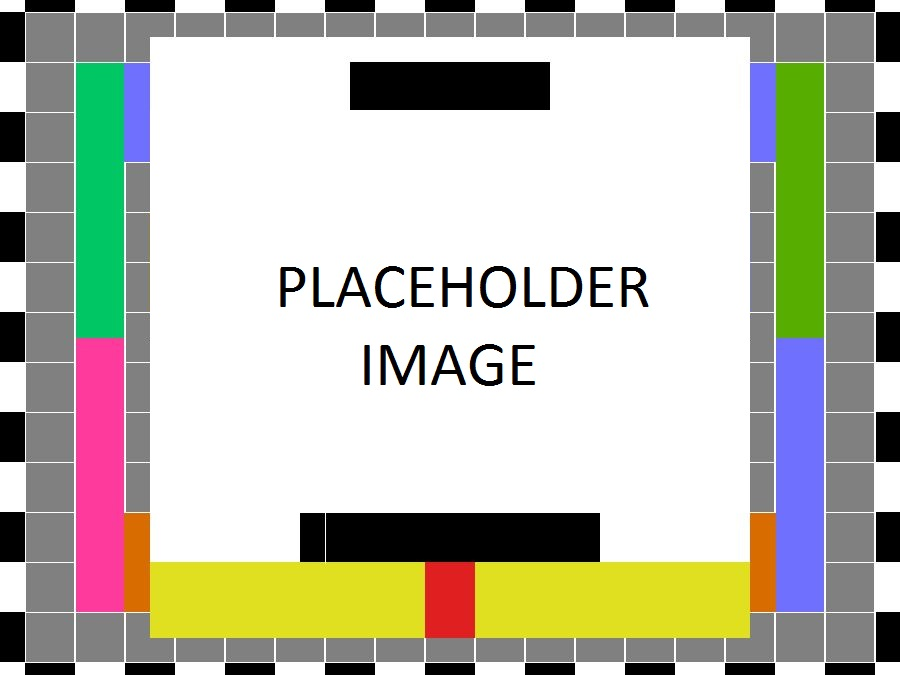
\includegraphics[width=0.60\textwidth]{images/test_image}
    \caption{X conceptual drawing}
\end{figure}
